\subsubsection{British Raj}

\paragraph{Outline}

WR, RMO. Super-efficient bonuses > south > west, north > east generally but depending on distribution. Games are either a) brawly T1/T2 fight - pick FTBs, clusters, combos or b) more positional and open. Large maps -> 4 spawns, want coverage, but as you play this more, you'll find out safety and coverage are illusions, some clusters and combos are so strong you just lose if you don't pick them.

\url{https://www.youtube.com/watch?v=MwQKbpBR4iY}
4x4, neutrals 2/2, wastelands 7/12, base: +5

\paragraph{Map Dynamics}
\url{https://imgur.com/JDjlxti} old picture

\begin{figure}[H]
  \centering
  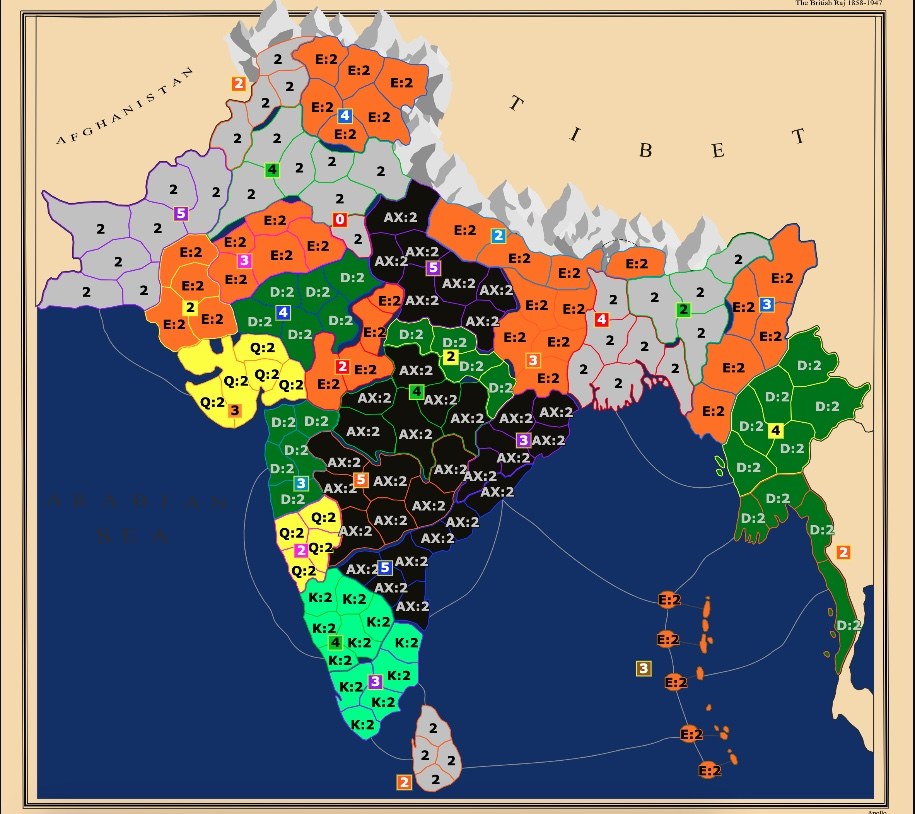
\includegraphics[width=0.8\textwidth]{Images/1800raj.jpg}
  \caption{Bonus Win Rates for Games with Overall Winner Rating >=1800 in British Raj (n=447) (AX>D>K>Q>E>-).}
  \label{raj_winrate_1800}
\end{figure}

\begin{itemize}
    \item The game generally revolves around the efficient +6s, when pickable.
    \item AX > 60\% Win Ratio. 
    \begin{enumerate}
        \item Purple +5 north is inefficient and very situational. You'll find the southern territories as good combo opportunities with \href{https://www.warzone.com/MultiPlayer?GameID=34620809}{yellow +3} or \href{https://www.warzone.com/MultiPlayer?GameID=36544268}{blue +5}. So a) as a combo pick for an FTB or 2TB into either expansion (\href{https://www.warzone.com/MultiPlayer?GameID=38099991}{Game}) into a relatively safe bonus or position to move north/east. The northern territories are generally a) for a combo for a safe region which is very rare, like \href{https://www.warzone.com/MultiPlayer?GameID=34314812}{here}, b) or to combo blue +2 FTB which I wouldn't recommend and c) as late counters with the idea of having contact later and moving in with a stack on turns 3-5 like \href{https://www.warzone.com/MultiPlayer?GameID=26183338}{here}.
        \item The efficient Orange +6 and Blue +6 shouldn't surprise you, the template revolves around these 2 bonuses (mainly). I've won with a triple blue +6 2TB featuring 2 wastelanded picks against Rufus \href{https://www.warzone.com/MultiPlayer?GameID=40543906}{here}. Really, the absolute first thing to think off in this template is making sure you cover those areas. 
        \item Green +4, Purple +3 and efficient Yellow +3 in the center all cover the best income regions and their WR depicts that.
    \end{enumerate}
    \item D > 55\% Win Ratio.
    \begin{enumerate}
        \item The blue +5 west shouldn't surprise you, it runs that region. It however is very difficult to defend from all directions (especially south and north).
        \item Light Blue +3 (North Bombay) is an interesting bonus in that it is very flexible. It can be used for a \href{https://www.warzone.com/MultiPlayer?GameID=33267988}{+4 FTB} if you like living dangerously. It can also be used for a \href{https://www.warzone.com/MultiPlayer?GameID=34086327}{purple +2 FTB}, \href{https://www.warzone.com/MultiPlayer?GameID=38248903}{combo with orange +6} \href{https://www.warzone.com/MultiPlayer?GameID=29469046}{combo for the +3 itself} and as a late counter to north. For example \href{https://www.warzone.com/MultiPlayer?GameID=40170077}{here}, ps picks it for a safe +6 bonus and uses it turn 5 to move north to Indore. Don't have a better example of it, but imagine if \href{https://www.warzone.com/MultiPlayer?GameID=33083890}{here} dco hit with a stack Indore anytime. The opponent's position collapses.
        \item The east yellow +4 and orange +2 are just generally good options for safe income. It can work because you have 4 spawns to cover the entire map, as such you can choose to have two cover/counter picks in the center and north + 2 picks east. However, you don't want to end up like \href{https://www.warzone.com/MultiPlayer?GameID=33152504}{here} with 0 options. Also you generally don't want to gamble two picks there vs a light green +2 FTB above it, due to how the +2 Bonus can walk to a double border within a turn.
    \end{enumerate}
    \item K > 50\% Win Ratio. Generally all around good bonuses with good borders.
    \item Q > 47 \% Win Ratio. 
    \begin{enumerate}
        \item Gujarat (orange +3) works best as a) FTB  with yellow +2 or by itself \href{https://www.warzone.com/MultiPlayer?GameID=39455294}{here} b) combo with +5 \href{https://www.warzone.com/MultiPlayer?GameID=38248903}{here} and \href{https://www.warzone.com/MultiPlayer?GameID=33795634}{here} c) late counter of solo pick only if you know what you are doing like \href{https://www.warzone.com/MultiPlayer?GameID=33003584}{here} (imo, toy around in WR with these late counters to test your limits. here you gotta go for it on T5 to bridge the income difference with the RF card, as it's 10vs15 and it's still quite a gamble).
        \item Purple +2 very popular option as an FTB or combo with neighboring bonuses.
    \end{enumerate}
    \item E >43\% Win Ratio. Don't get me wrong, these bonuses aren't necessarily bad, most of the times they are overpicked in positions where they shouldn't. Prioritize smaller bonuses when you have early fights. Prioritize really safe income like the north blue +4 when you need the safe income like \href{https://www.warzone.com/MultiPlayer?GameID=39978166}{here}
\end{itemize}

\paragraph{Picking Logic}

I personally separate British Raj distributions at first glance within seconds into a) brawly T1-T2 fight distributions and b) more open distributions where position matters more. For example \href{https://www.warzone.com/MultiPlayer?GameID=39978166}{here} I embrace that the game revolves around the blue +6 FTB. It is 7 territories for +6 income that's very easy to defend from all fronts and has good proximity to other bonuses. What can compare against it? Can the east +2 FTB with that inefficient red +4 compare? 
\begin{itemize}
    \item 3 Picks for the +6 come at 7 territories for 6 income or 13 territories for 10 income later.
    \item In the east it's 4 territories for 2 income and  10 territories for 6 income later.
\end{itemize}
The difference is astronomical.

\begin{wrapfigure}{r}{0.35\textwidth}
    \centering
  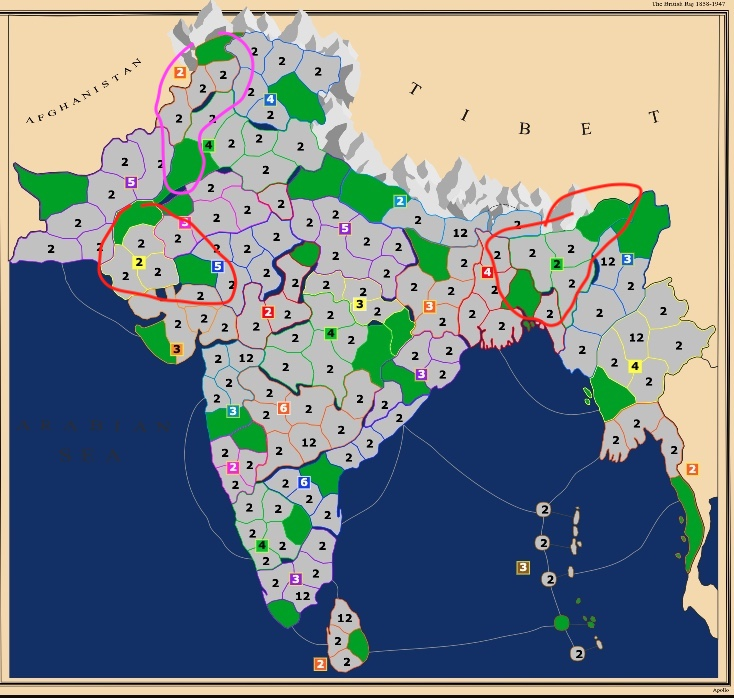
\includegraphics[width=0.35\textwidth]{Images/raj_game.jpg}
  \caption{British Raj Distribution 7ate9 vs FiveStarGeneral}
  \label{raj_game_example}
\end{wrapfigure}

We've realized it's all about that +6 Bonus, we realize we will have contact/fight on Turn 1, the latest Turn 2, so I need to pick in a way that gives me the edge there. (Figure \ref{raj_game_example}). Start discarding picks based on that. 
\begin{itemize}
    \item All those slow +4 and +5 bonuses picks should be completely useless if I have contact and fights around the blue +6 early. 
    \item Some +3 combos maybe can work, like Orange +3 combo west, but the expansion is extremely slow, and it will need from me 4-6/10 of my deployments on Turns 1-2 which if I contest the blue +6 it's hard to find.
\end{itemize}

We suddenly are left only with blue +6, picks around it, and the three FTBs. The board is simplified. Now we can plan a couple of picksets and go for something that's comfortable / wins against others. My first pick covers both FTBs north. My 1/2/3 gives me an extremely safe region with a cover spawn in the center. If I get 123 + one of my 5-8 I win. If I get 1/2 and 2 of my center spawns, I feel comfortable in winning, unless it's 1/2/5/7. If I get 2/3 and 2 center spawns, it sucks a bit. The more you look into it, you can find holes in my pickset, but I figured my opponent won't see this triple safe into cover center strategy and I just went for it. In reality, the central - efficient bonus - region is so unbelievably good that a lot of British Raj in theory should be very brawly, and you can chceck out some of the seasonal game son it like \href{https://www.warzone.com/MultiPlayer?GameID=36358933}{here}, \href{https://www.warzone.com/MultiPlayer?GameID=36442714}{here} and \href{https://www.warzone.com/MultiPlayer?GameID=36276373}{here}. Safety is an illusion. It doesn't matter in this template as much as you think. 
\\
\\
In more open distributions, you have some flexibility and options. These surface more often than not when there aren't broken combos or FTBs, as for example \href{https://www.warzone.com/MultiPlayer?GameID=40619051}{here} everything appears equally good. There's the orange +6 that's extremely easy to cover and then there's decent bonuses everywhere. Generally in such positions I opt for combo picking safe regions with positional advantage and better expansion. You'll see in the example above, we both pick very differently with specific ideas in set. 
\begin{itemize}
    \item Bechaa covers the orange +6 and entire center with his 1st pick. If he loses that, he always goes down to 5-7, so he gets minimum one of 5-7. Worst case for him he gets 2/3/4/7. (Cannot get 2/3/4/8). His strategy relies heavily on 
    \begin{enumerate}
        \item a) 1/2/3 + cover to fight. 1-3 pair nicely if needed for expansion between them.
        \item b) 2/3/4 + cover on 5-6-7 to use 2/3 ftb to fight west and 5-7 to fight center.
    \end{enumerate}
    \item I throw a 1/2 in the orange +6 to cover the combo and the FTB, 3/5 west for coverage in a great region, 4 center and 678 east. In retrospect, very poorly thought picks without a strategy in mind, but flexible nonetheless.
\end{itemize}

There is no right or wrong, you can win with a suboptimal pickset that perfectly counters something else. I generally favour all around flexible picks here due to the luck coming from RMO and WR.

\paragraph{Gameplay}
% early, mid, cards

I'll take the previous example vs Bechaa \href{https://www.warzone.com/MultiPlayer?GameID=40619051}{here} in a game I should've lost. I see WR and British Raj as an extension as a template where you should expand towards the opponent. Turn 2 I use recon south. I don't need to use the recon in the light blue +3 that can counter later my 1/2 FTB. Him having that doesn't influence the outcome of the game, chances are he would deploy to break my bonus more than I invested to get the bonus to begin with. I need to know if he spawned south to a) limit his starting options and b) know if I should head south or not. No green +4 south -> no blue +6, only a +3, noone cares. I move east in the +6 becomes it's magnificently overpowerful, easy to defend and my path to reaching his income.
\\
\\
End of Turn 4 I get hit by stack attack north and am 12vs13 Income. Need to bait a lot of deployments by him North and flank south. Potentially even fake the blue +5 and threaten his income there.
\\
\\
Check the position end of T5. I am down 22 movable armies, but Bechaa deployed +27 across two turns in order to break +3 income that I got by investing +7 armies. Don't feel intimidated by the position as Bechaa is not in fact winning here. The position is very poisonous for him, He doesn't know if I completed the +5 in his face, he has over-committed in the wrong direction and if he loses RMO twice, I threaten his income north. This game illustrates perfectly the power of pivoting. Use fog to your advantage, don't over-commit, count and play to win the game, not just break a +3 bonus.
\\
\\
Game starts with a recon and a blockade. Recon's existence comes with the ability to pick in a way that forces using recon in a cluster T1. 
\begin{itemize}
    \item Turn 5 you can use first RF +5 (4 pieces)
    \item Turn 6 for OD (5 pieces)
    \item Turn 7 for OP (6 pieces)
\end{itemize}

